%% Before processing this LaTeX file (LaTeX2e), make sure that the file
%% TCAM.cls is in the same folder. The file TCAM.cls can be obtained from
%% https://tcam.sbmac.org.br.


%\documentclass[english]{TCAM} % Use for manuscripts written in English
\documentclass[brazil]{TCAM} % Usar para manuscritos escritos em Português


%%%%%%%%%%%%%%%%%%%%%%%%%%%%%%%%%%%%%%%%%%%%%%%%%%%%%%%%%%%%%%%%%%%%%%%%%%%%%%%%%%%%%%%%%%%%%%%%%%%%%
% Attention:
% This file uses UTF-8 encoding.
%%%%%%%%%%%%%%%%%%%%%%%%%%%%%%%%%%%%%%%%%%%%%%%%%%%%%%%%%%%%%%%%%%%%%%%%%%%%%%%%%%%%%%%%%%%%%%%%%%%%%

\usepackage[utf8]{inputenc} % UTF-8 encoding

\usepackage{multirow}
\usepackage{array}
\usepackage{url}
\usepackage{graphicx}
\usepackage{subfigure}
\usepackage{lineno} % to display line numbers
\linenumbers

\usepackage{listingsutf8} % for code listings

\lstdefinestyle{mystyle}{
basicstyle=\ttfamily\footnotesize,
breakatwhitespace=false,
breaklines=true,
captionpos=b,
keepspaces=true,
showspaces=false,
showstringspaces=false,
showtabs=false,
tabsize=2
}

\lstset{style=mystyle}

%********************************************************
% LIST ALL PACKAGES REQUIRED BY YOUR PAPER HERE
%********************************************************
\usepackage{framed}
\usepackage{tikz}

%********************************************************
% PAPER INFORMATION
%********************************************************

\title{Cisalhamento antiplano em um compósito bifásico: comparação entre Diferenças
Finitas, Elementos Finitos e PINNs.}

\runningtitle{Análise numérica de compósito bifásico}

\author{Bianca Bonfim, Pedro Cruz, Richard Francis
}
%\aff{Affiliations should be omitted to ensure a double-blind review process. After review and acceptance, the final manuscript must include a full list of authors, affiliations with addresses, email, and mandatory ORCID.}, %
%*********************************************************
% Use this template to add author's names after the
% double-blind review process.
%*********************************************************
% Anonymous Second Author%
% \aff{Department of Applied Mathematics and Statistics, ICMC, University of São Paulo, Av. Trabalhador São-carlense, 400, 13566-590, São Carlos, SP, Brazil -- E-mail: tcam@sbmac.org.br https://orcid.org/xxxx-xxxx-xxxx-xxxx} %
%}

\abstracttcam{Este trabalho apresenta um estudo comparativo entre três abordagens numéricas distintas — o Método de Diferenças Finitas (MDF), o Método de Elementos Finitos (MEF) e as Redes Neurais Informadas pela Física (PINNs) — aplicadas à análise de cisalhamento antiplano em um compósito bifásico com célula de inclusão. Os resultados indicam uma convergência consistente entre os três métodos na estimativa do módulo de cisalhamento. No entanto, a análise revelou que o MEF apresenta precisão superior na captura das tensões de interface. As PINNs, embora eficazes na representação do deslocamento global, demonstraram maior dificuldade em resolver as descontinuidades de gradiente nas quinas da inclusão. O estudo conclui que, enquanto os métodos de discretização clássicos permanecem mais precisos para problemas determinísticos de interface, as PINNs oferecem um paradigma flexível e livre de malha para a homogeneização computacional.}

\keywords{Cisalhamento antiplano, Diferenças Finitas, Elementos Finitos, PINN}

%\acknowledgments{The acknowledgments section is optional. Please omit it in the submission version to ensure a double-blind peer-review process.}


%***************************************************************
% INFORMATIONS IN ENGLISH - MANDATORY WHEN WRITING IN PORTUGUESE
% CAN BE OMITTED WHEN WRITING THE MANUSCRIPT IN ENGLISH
%
\titleenglish{Antiplane Shear in a two-phase composite: comparasion between Finite Differences, Finite Elements and PINNs}

\abstracttcamenglish{This paper presents a comparative study of three distinct numerical approaches—the Finite Difference Method (FDM), the Finite Element Method (FEM), and Physics-Informed Neural Networks (PINNs)—applied to the analysis of anti-plane shear in a two-phase composite with an inclusion cell. The results indicate consistent convergence among the three methods in estimating the shear modulus. However, the analysis revealed that the FEM offers superior accuracy in capturing interface stresses. While effective at representing global displacement, PINNs demonstrated greater difficulty in resolving gradient discontinuities at the inclusion corners. The study concludes that, although classical discretization methods remain more accurate for deterministic interface problems, PINNs offer a flexible, mesh-free paradigm for computational homogenization.}

\keywordsenglish{Antiplane Shear, Finite-Difference Method, Finite-Elements Method, PINN }

%***************************************************************


\begin{document}

%********************************************************

\maketitle

%********************************************************

\section{Introdução}

Diversos materiais compósitos apresentam uma célula de inclusão onde se torna necessário conhecer as regiões de concentração de tensão e possíveis pontos de falha. Podemos ver aplicações desses materiais em biomateriais, cerâmicas, concretos e materiais porosos.
A formulação antiplana reduz o problema tridimensional a um problema bidimensional preservando aspectos físicos essenciais.

Neste trabalho, faremos uma comparação das soluções obtidas pelos métodos de Diferenças Finitas, Elementos Finitos e a solução obtida através da PINN. Em Diferenças Finitas, as derivadas parciais podem ser expressas através de combinação linear de seus nós vizinhos resultando em um sistema de equações lineares ao final \cite{lin2021simulation}\cite{leveque2007}. Em Elementos Finitos, usa-se a formulação clássica aplicando o método de resíduos ponderados para encontrar a formulação fraca e o método de Galerkin para as funções de interpolação resultando também em um sistema linear \cite{logan}. Já na simulação obtida com uso da PINN,tem-se uma abordagem de aprendizado profundo que integra as leis da física diretamente na função de perda da rede neural.

O objetivo principal é avaliar a eficácia de cada método na captura dos campos locais e na estimativa do módulo de cisalhamento efetivo do compósito, confrontando a eficiência das discretizações clássicas com a flexibilidade da inteligência artificial informada pela física


\section{Descrição física do problema}

O problema de cisalhamento antiplano descreve o comportamento mecânico de um corpo prismático longo, cujo comprimento na direção axial é muito superior às dimensões de sua seção transversal. Sob essa hipótese, admite-se que o único deslocamento não nulo ocorre na direção do eixo do corpo (fora do plano da seção), enquanto os deslocamentos no plano da seção são nulos. Além disso, supõe-se que esse deslocamento axial depende apenas das coordenadas $(x,y)$ da seção transversal, sendo invariante ao longo do eixo. Dessa forma, o estado tridimensional de deformação reduz-se a um problema escalar bidimensional para o campo de deslocamento $w(x,y)$, preservando os aspectos físicos essenciais do problema original \cite{lin2021simulation}.

Nessa configuração, as únicas componentes não nulas de tensão são as de cisalhamento associadas aos planos $xz$ e $yz$, denotadas por $\tau_{xz}$ e $\tau_{yz}$. Na ausência de forças de corpo, o equilíbrio mecânico exige que a divergência do campo de tensões seja nula, o que conduz diretamente à equação governante apresentada na seção seguinte.

O corpo considerado é um material compósito bifásico, representado por uma célula representativa composta por uma matriz que envolve uma inclusão central. A matriz e a inclusão possuem módulos de cisalhamento distintos, $G_m$ e $G_i$, de modo que a propriedade material $G(x,y)$ é descontínua através da interface entre as duas fases. Essa descontinuidade é a principal fonte de complexidade física do problema: na interface, exige-se simultaneamente a continuidade do deslocamento $w$ e o equilíbrio do fluxo de tensão normal, $G\,\partial w/\partial n$, enquanto o gradiente do deslocamento sofre um salto. Como consequência, surgem concentrações de tensão, particularmente acentuadas nas quinas da inclusão, regiões frequentemente associadas ao início de falhas em materiais reais.

Ao corpo impõe-se um cisalhamento macroscópico simples, que induz um campo de deslocamento médio através da célula. O interesse prático é duplo: por um lado, deseja-se conhecer os campos locais de tensão, identificando as regiões de concentração e os possíveis pontos de falha; por outro, busca-se estimar o módulo de cisalhamento efetivo $G_{ef}$ do compósito, isto é, a propriedade homogeneizada que descreve o comportamento médio do material heterogêneo como se fosse um meio equivalente. Esse procedimento de obtenção de propriedades efetivas a partir da microestrutura é o objeto da homogeneização computacional \cite{geers2010multiscale} e constitui o elo entre a descrição microscópica da célula e o comportamento macroscópico do compósito em aplicações como biomateriais, cerâmicas, concretos e materiais porosos.


\section{Formulação Matemática}
Nesse capítulo, iremos abordar a modelagem matemática do problema tratado.
Dada uma célula representativa de um material compósito. Considere a matriz que possui módulo de cisalhamento $G_m$ enquanto uma inclusão central possui módulo de cisalhamento $G_i$.

Considere o domínio quadrado:
\begin{equation*}
    \Omega = [0,L] \times [0,L]
\end{equation*}

No centro do domínio há uma inclusão quadrada definida por:
\begin{equation*}
    \Omega_i = \Big[\dfrac{L}{2}-a, \dfrac{L}{2}+a\Big] \times \Big[\dfrac{L}{2}-a, \dfrac{L}{2}+a\Big]
\end{equation*}

A matriz é definida por:
\begin{equation*}
    \Omega_m = \Omega \setminus \Omega_i.
\end{equation*}

O módulo de cisalhamento é:
\begin{equation*}
    G(x,y)=
\begin{cases}
G_i, & (x,y)\in\Omega_i,\\[2mm]
G_m, & (x,y)\in\Omega_m.
\end{cases}
\end{equation*}

Iremos utilizar para os cálculos numéricos os valores de:

\begin{equation*}
    L = 1,
\qquad
a = 0.15,
\qquad
G_m = 1,
\qquad
G_i = 5.
\end{equation*}

\subsection{Modelo matemático}

O deslocamento antiplano é representado por $w(x,y)$. A equação de equilíbrio é:
\begin{equation}
    -\nabla \cdot \bigl(G(x,y)\nabla w(x,y)\bigr)=0,
\qquad
(x,y)\in\Omega.
\label{eq}
\end{equation}

As tensões de cisalhamento são:

\[
\tau_{xz}
=
G(x,y)\frac{\partial w}{\partial x},
\]

\[
\tau_{yz}
=
G(x,y)\frac{\partial w}{\partial y}.
\]

\subsection{Condições de Contorno}

Imponha um cisalhamento macroscópico simples:
\begin{eqnarray}
    w(0,y)&= 0, \\
    w(L,y)&= \gamma L
\end{eqnarray}

onde \(\gamma\) é a deformação de cisalhamento imposta, ou seja,  temos nesse caso condição de contorno de Dirichlet.

Nas bordas superior e inferior, impõe-se condição de fluxo nulo:
\begin{eqnarray}
    \frac{\partial w}{\partial y}(x,0)=0 \\
    \frac{\partial w}{\partial y}(x,L)=0
    \label{contorno}
\end{eqnarray}

Neste caso, temos também condição de contorno de Neumann.
%********************************************************
\section{Método de diferenças finitas}

Considere a equação governante do problema de cisalhamento antiplano apresentada em \eqref{eq}.
Expandindo a equação, teremos:

\begin{equation*}
- \frac{\partial}{\partial x}
\left(
G(x,y) \frac{\partial w}{\partial x}
\right)
-
\frac{\partial}{\partial y}
\left(
G(x,y) \frac{\partial w}{\partial y}
\right)
=0.
\end{equation*}

Essa formulação é amplamente empregada na análise de problemas de cisalhamento antiplano em materiais heterogêneos contendo inclusões \cite{lin2021simulation}.

O domínio é discretizado por uma malha uniforme de espaçamento $h$,
contendo $n$ nós em cada direção. Os nós da malha são identificados
pelos índices $i,j=0,\ldots,n$.

Para preservar adequadamente os fluxos nas interfaces entre materiais distintos, os coeficientes são avaliados nos pontos médios entre nós.
A discretização é realizada na forma conservativa, aproximando inicialmente as tensões de cisalhamento nas interfaces entre os volumes de controle e, em seguida, aproximando a divergência dessas tensões por diferenças centrais.

\subsection{Discretização da Equação Governante}
Define-se a tensão de cisalhamento na direção $xz$ por:
\begin{equation}
     \tau_{xz}=G\dfrac{\partial w}{\partial x}
\label{4.2}
\end{equation}

Utilizando aproximações por diferenças finitas centrais de segunda ordem \cite{leveque2007}:
$$
\frac{\partial \tau_{xz}}{\partial x} \approx \dfrac{\tau_{xz_{i+1/2,j}} - \tau_{xz_{i-1/2,j}}}{h}
$$
E
\begin{equation}
\begin{aligned}
\tau_{xz\,\,i+\frac12,j}
&=
G_{i+\frac12,j}
\frac{w_{i+1,j}-w_{i,j}}{h},
\\[2mm]
\tau_{xz\,\,i-\frac12,j}
&=
G_{i-\frac12,j}
\frac{w_{i,j}-w_{i-1,j}}{h}.
\end{aligned}
\label{4.3}
\end{equation}

Substituindo as Equações \eqref{4.3} em \eqref{4.2}, obtém-se:
\begin{equation}
    \frac{\partial}{\partial x}
\left(
G(x,y) \frac{\partial w}{\partial x}
\right) = \frac{G_{i+\frac12,j}
{(w_{i+1,j}-w_{i,j})} - G_{i-\frac12,j}
(w_{i,j}-w_{i-1,j})}{h^2}
\end{equation}

Analogamente, discretizando em $y$, teremos:
\begin{equation*}
    \frac{\partial}{\partial y}
\left(
G(x,y) \frac{\partial w}{\partial y}
\right) = \frac{G_{i,j+\frac12}
{(w_{i,j+1}-w_{i,j})} - G_{i,j-\frac12}
(w_{i,j}-w_{i,j-1})}{h^2}
\end{equation*}

E assim, a discretização final é dada por:
\begin{equation*}
\begin{aligned}
&\Bigl(
G_{i+\frac{1}{2},j}w_{i+1,j}
+G_{i-\frac{1}{2},j}w_{i-1,j}
+G_{i,j+\frac{1}{2}}w_{i,j+1}
+G_{i,j-\frac{1}{2}}w_{i,j-1}
\Bigr) \\
&-
\Bigl(
G_{i+\frac{1}{2},j}
+G_{i-\frac{1}{2},j}
+G_{i,j+\frac{1}{2}}
+G_{i,j-\frac{1}{2}}
\Bigr)w_{i,j}
=0.
\end{aligned}
\end{equation*}
Observa-se que a equação discreta relaciona cada nó da malha aos seus
quatro vizinhos adjacentes nas direções horizontal e vertical,
caracterizando um stencil de cinco pontos. Essa estrutura é utilizada na
montagem do sistema linear associado ao problema.

A utilização da média harmônica permite representar adequadamente a
transição entre materiais com propriedades distintas, preservando a
continuidade do fluxo de tensões através da interface. Portanto tem-se que:
\begin{equation}
     G_{i+\frac12,j}= \dfrac{2G_{i,j}G_{i+1,j}}{G_{i,j}+G_{i+1,j}}
\end{equation}


\subsection{Discretização das Condições de Contorno}

As condições de Dirichlet são impostas diretamente nos nós pertencentes ao contorno. Assim,
\begin{equation*}
    w_{0,j}=0
\end{equation*}
e
\begin{equation*}
    w_{n,j}=\gamma L
\end{equation*}

Esses valores são incorporados diretamente ao sistema linear.

Nas fronteiras superior e inferior do domínio são impostas condições de Neumann homogêneas, correspondentes à ausência de fluxo de tensão de cisalhamento através do contorno. Matematicamente,

\begin{equation*}
\frac{\partial w}{\partial y}=0.
\end{equation*}

Como a tensão de cisalhamento é dada por

\begin{equation}
\tau_{yz}=G\frac{\partial w}{\partial y},
\end{equation}

segue que

\begin{equation*}
\tau_{yz}=0
\end{equation*}

nas fronteiras superior e inferior.

Para discretizar essa condição mantendo a ordem de precisão do esquema, utiliza-se uma aproximação por diferenças centrais.
Na fronteira inferior $(j=0)$, utilizando diferenças centrais e introduzindo um nó fantasma, obtém-se

\begin{equation*}
\frac{w_{i,1}-w_{i,-1}}{2h}=0,
\end{equation*}

de onde resulta

\begin{equation*}
w_{i,1}=w_{i,-1}.
\end{equation*}

De maneira análoga, na fronteira superior,

\begin{equation*}
\frac{w_{i,n+1}-w_{i,n-1}}{2h}=0,
\end{equation*}

o que fornece

\begin{equation*}
w_{i,n+1}=w_{i,n-1}.
\end{equation*}

\subsection{Montagem do sistema linear}

A aplicação da discretização em todos os nós internos da malha,
juntamente com as condições de contorno, resulta em um sistema linear
de equações da forma

\begin{equation*}
A\mathbf{w}=\mathbf{b},
\end{equation*}

em que $A$ é a matriz dos coeficientes provenientes da discretização,
$\mathbf{w}$ é o vetor das incógnitas nodais e $\mathbf{b}$ incorpora
as contribuições das condições de contorno.

Cada linha da matriz $A$ corresponde à equação discreta associada a um
nó da malha. Devido ao stencil de cinco pontos empregado, a matriz
resultante é esparsa, contendo coeficientes apenas para os vizinhos
imediatos de cada nó.
%%%%%%%%%%%%%%%%%%%%%%%%%%%%%%%%%%%%%%%%%%%%

\section{Método de elementos finitos}

Baseando-se no método de resíduos ponderados e aplicando a formulação que vemos em \cite{logan}, multiplicamos a equação por uma função teste $v$ e aplica-se a integração no domínio, tal que:

\begin{equation*}
\int_{\Omega} v \, \nabla \cdot (G \nabla w)\, d\Omega = 0.
\end{equation*}

Aplicando o teorema da divergência, resulta

\begin{equation*}
\int_{\Omega} G \nabla v \cdot \nabla w \, d\Omega
-
\int_{\Gamma}
v \, (G\nabla w \cdot \mathbf{n})
\, d\Gamma
=
0,
\end{equation*}

em que $\mathbf{n}$ representa o vetor normal unitário ao contorno $\Gamma$.

Considerando condições de contorno  homogêneas dadas em \eqref{contorno}, tem-se:

\begin{equation*}
G\nabla w \cdot \mathbf{n}=0
\qquad \text{em } \Gamma_N,
\end{equation*}

então o termo de contorno é anulado, restando

\begin{equation}
\int_{\Omega}
G \nabla v \cdot \nabla w
\, d\Omega
=
0.
\label{eq:forma_fraca}
\end{equation}

A Equação \eqref{eq:forma_fraca} constitui a formulação fraca do problema.

Fazendo a discretização para $n$ pontos, devemos então encontrar coeficientes $w_i$ e funções de interpolação $N_i$ para encontrar uma aproximação tal que:
\begin{equation}
    w(x,y)
=
\sum_{i=1}^{n}
N_i(x,y)\, w_i.
\label{eq:aprox_w}
\end{equation}

 Adotando o método de Galerkin, a função teste é interpolada utilizando as mesmas funções de forma.
\begin{equation}
v(x,y)
=
\sum_{i=1}^{n}
N_i(x,y)\, v_i.
\label{eq:aprox_v}
\end{equation}

As funções $N_i$ são escolhidas de forma que $N_i(x_j,y_j)=\delta_{ij}$, sendo $\delta$ a função delta de Kroenecker.

Substituindo as Equações \eqref{eq:aprox_w} e \eqref{eq:aprox_v}
em \eqref{eq:forma_fraca}, teremos:

\begin{equation*}
    \int_{\Omega}
G
\left(
\sum_{i=1}^{n}
\nabla N_i\, v_i
\right)
\cdot
\left(
\sum_{j=1}^{n}
\nabla N_j\, w_j
\right)
\, d\Omega
=0.
\end{equation*}


Como \(v_i\) e \(w_j\) são coeficientes nodais constantes, eles podem ser retirados da integral, resultando em

\begin{equation*}
\sum_{i=1}^{n}
\sum_{j=1}^{n}
v_i
\left(
\int_{\Omega}
G\,\nabla N_i\cdot\nabla N_j
\, d\Omega
\right)
w_j
=0.
\end{equation*}

Define-se:
\begin{equation*}
    K_{ij} = \int_{\Omega} G \nabla N_{i} \cdot \nabla N_j d \Omega
\end{equation*}

Organizando as derivadas em forma matricial:
\[
B=
\begin{bmatrix}
\dfrac{\partial N_1}{\partial x} &
\dfrac{\partial N_2}{\partial x} &
\dots &
\dfrac{\partial N_n}{\partial x}
\\[3mm]
\dfrac{\partial N_1}{\partial y} &
\dfrac{\partial N_2}{\partial y} &
\dots &
\dfrac{\partial N_n}{\partial y}
\end{bmatrix}
\]

Logo,
$$\mathbf{K}=\int_{\Omega}\mathbf{B}^TG\mathbf{B} d\Omega$$

%********************************************************
\section{PINN}

\subsection{Metodologia e Arquitetura}

As \textit{Physics-Informed Neural Networks} (PINNs) constituem uma abordagem em
que uma rede neural $\mathcal{N}_\theta(x,y)$ aproxima diretamente o campo de
deslocamento $w(x,y)$, ajustando seus parâmetros $\theta$ de forma a minimizar o
resíduo da equação diferencial parcial governante e das condições de contorno. A principal vantagem é a ausência de malha: as derivadas
são obtidas por diferenciação automática (\textit{autograd}), o que as torna exatas
no sentido computacional.

Como $G(x,y)$ é descontínuo na interface $\partial\Omega_i$, uma única rede
apresenta dificuldades em capturar o salto de gradiente. Contudo, $G$ é constante
dentro de cada subdomínio; portanto, a equação \eqref{eq} se reduz à equação de
Laplace em cada fase:
\begin{equation}
    \nabla^2 w = 0, \qquad (x,y) \in \Omega_m \cup \Omega_i.
\end{equation}

Toda a física não-trivial fica concentrada na interface $\partial\Omega_i$. Adota-se
então a estratégia de \textit{domínio decomposto}: duas redes independentes,
\begin{equation*}
    \mathcal{N}_m^{\theta_m}(x,y) \approx w\big|_{\Omega_m}, \qquad
    \mathcal{N}_i^{\theta_i}(x,y) \approx w\big|_{\Omega_i},
\end{equation*}
acopladas pelas condições de interface.

Cada rede é um perceptron multicamadas (MLP) com:
\begin{itemize}
    \item 5 camadas ocultas de 48 neurônios cada;
    \item função de ativação $\tanh$;
    \item camada de saída linear com 1 neurônio;
    \item entrada $(x,y)$ normalizada para $[-1,1]^2$ via
          $\boldsymbol{\xi} = 2(x,y)/L - 1$.
\end{itemize}

\subsection{Treinamento e função de perda}

A função de perda total é
\begin{equation}
    \mathcal{L}(\theta_m, \theta_i)
    = \lambda_{\text{EDP}}\,\mathcal{L}_{\text{EDP}}
    + \lambda_{\text{CC}}\,\mathcal{L}_{\text{CC}}
    + \lambda_{I}\,\mathcal{L}_{I},
\end{equation}
com $\lambda_{\text{EDP}} = 1$, $\lambda_{\text{CC}} = \lambda_I = 10$.

\paragraph{Resíduo da EDP.}
O resíduo de Laplace é avaliado em pontos de colocação amostrados
aleatoriamente em cada subdomínio:
\begin{equation}
    \mathcal{L}_{\text{EDP}}
    = \frac{1}{N_m}\sum_{k=1}^{N_m}
      \bigl(\nabla^2 \mathcal{N}_m(\mathbf{x}_k^m)\bigr)^2
    + \frac{1}{N_i}\sum_{k=1}^{N_i}
      \bigl(\nabla^2 \mathcal{N}_i(\mathbf{x}_k^i)\bigr)^2.
\end{equation}

\paragraph{Condições de contorno.}
Para as fronteiras do domínio (pertencentes à matriz):
\begin{equation}
\begin{aligned}
    \mathcal{L}_{\text{CC}}
    &= \frac{1}{N_b}\sum_k \mathcal{N}_m(0,y_k)^2
    + \frac{1}{N_b}\sum_k \bigl(\mathcal{N}_m(L,y_k)-\gamma L\bigr)^2 \\
    &\quad
    + \frac{1}{N_b}\sum_k \left(\frac{\partial \mathcal{N}_m}{\partial y}
      \bigg|_{y=0}\right)^2
    + \frac{1}{N_b}\sum_k \left(\frac{\partial \mathcal{N}_m}{\partial y}
      \bigg|_{y=L}\right)^2.
\end{aligned}
\end{equation}

\paragraph{Condições de interface.}
Na interface $\partial\Omega_i$ impõem-se continuidade do deslocamento e equilíbrio
do fluxo de tensão:
\begin{equation}
\begin{aligned}
    \mathcal{L}_{I}
    &= \frac{1}{N_f}\sum_k
      \bigl(\mathcal{N}_m(\mathbf{x}_k^f) - \mathcal{N}_i(\mathbf{x}_k^f)\bigr)^2 \\
    &\quad + \frac{1}{N_f}\sum_k
      \bigl(G_m\,\partial_n \mathcal{N}_m(\mathbf{x}_k^f)
           - G_i\,\partial_n \mathcal{N}_i(\mathbf{x}_k^f)\bigr)^2,
\end{aligned}
\end{equation}
onde $\partial_n = \mathbf{n}\cdot\nabla$ é a derivada na direção normal exterior à
inclusão, calculada analiticamente para cada face do quadrado.

Os pontos são amostrados aleatoriamente com semente fixa ($s = 42$):
\begin{itemize}
    \item $N_m = 4\,000$ pontos no interior de $\Omega_m$ (matriz);
    \item $N_i = 4\,000$ pontos no interior de $\Omega_i$ (inclusão);
    \item $N_b = 400$ pontos em cada fronteira externa (esquerda, direita, topo, base);
    \item $N_f = 600$ pontos na interface $\partial\Omega_i$ (150 por lado do quadrado).
\end{itemize}

Os parâmetros são otimizados pelo algoritmo Adam \cite{kingma2015adam} com taxa de
aprendizado $\eta = 10^{-3}$ ao longo de $4\,000$ épocas. As duas redes são
treinadas simultaneamente; os gradientes de $\mathcal{L}_I$ se propagam por ambas,
forçando o acoplamento na interface. A semente aleatória é fixada para garantir
reprodutibilidade.

\subsection{Avaliação e cálculo das tensões}

Após o treinamento, as redes são avaliadas numa malha regular $(N+1)\times(N+1)$
com $N = 80$. O campo de deslocamento é obtido selecionando a rede correspondente
a cada fase:
\begin{equation*}
    w(x_k, y_k) =
    \begin{cases}
        \mathcal{N}_i(x_k,y_k), & (x_k,y_k) \in \Omega_i, \\
        \mathcal{N}_m(x_k,y_k), & (x_k,y_k) \in \Omega_m.
    \end{cases}
\end{equation*}

As tensões são computadas pelo gradiente exato de cada rede no seu próprio
subdomínio via \textit{autograd}, evitando a diferenciação do campo costurado
(que introduziria erros espúrios na interface):
\begin{equation*}
    \tau_{xz} = G\,\nabla_x \mathcal{N}\big|_{\text{subdomínio}}, \qquad
    \tau_{yz} = G\,\nabla_y \mathcal{N}\big|_{\text{subdomínio}}.
\end{equation*}

O módulo efetivo é estimado por:
\begin{equation*}
    G_{ef} = \frac{\langle \tau_{xz} \rangle}{\gamma}.
\end{equation*}

%********************************************************
\section{Resultados numéricos}

Os resultados a seguir são decorrentes da solução numérica aplicada através da linguagem de programação Python com as bibliotecas \texttt{NumPy},
\texttt{SciPy} e \texttt{PyTorch}, e executados com os parâmetros resumidos na
Tabela~\ref{tab:params}.

\begin{table}[h]
\centering
\caption{Parâmetros de discretização e treinamento utilizados em cada método.}
\label{tab:params}
\begin{tabular}{lll}
\hline
\textbf{Parâmetro} & \textbf{MDF / MEF} & \textbf{PINN} \\
\hline
Tamanho da malha de solução    & $N = 80$ ($81{\times}81$ nós) & $N = 80$ (avaliação) \\
Incógnitas do sistema linear   & $6\,561$                      & ---                  \\
Pontos interiores (matriz)     & ---                           & $4\,000$             \\
Pontos interiores (inclusão)   & ---                           & $4\,000$             \\
Pontos de contorno externo     & ---                           & $400$ por face       \\
Pontos de interface            & ---                           & $600$                \\
Épocas de treinamento          & ---                           & $4\,000$             \\
Otimizador                     & ---                           & Adam, $\eta=10^{-3}$ \\
Arquitetura                    & ---                           & MLP $5{\times}48$, $\tanh$ \\
\hline
\end{tabular}
\end{table}

No MDF, os coeficientes nas faces da malha são calculados pela média harmônica dos
valores nodais adjacentes, o que preserva a continuidade do fluxo de tensão na
interface matriz--inclusão. No MEF, o valor de $G$ é atribuído por elemento a partir
do centroide, usando elementos quadrilaterais Q4 com quadratura de Gauss $2{\times}2$.

\subsection{Validação contra solução analítica}

Antes de analisar o caso oficial (inclusão quadrada), os solvers foram validados
contra a solução analítica para inclusão \emph{circular} de raio $a = 0{,}15$
com $G_i = 10$. A solução exata em coordenadas polares centradas na inclusão é:
\begin{equation*}
    w(r,\theta) =
    \begin{cases}
        \dfrac{2G_m}{G_i+G_m}\,\gamma\,r\cos\theta + \gamma\,c_x,
        & r < a, \\[4pt]
        \gamma\,r\cos\theta
        + \gamma\,a^2\,\dfrac{G_m-G_i}{G_m+G_i}\,\dfrac{\cos\theta}{r}
        + \gamma\,c_x,
        & r \ge a,
    \end{cases}
\end{equation*}
onde $c_x = L/2$ é a coordenada $x$ do centro. O MDF com $N = 120$
($121{\times}121$ nós) produziu um erro relativo em norma $L^2$ inferior a $1\%$
no interior do domínio ($0{,}2 \le x, y \le 0{,}8$), confirmando a correta
implementação.

Um estudo de convergência foi realizado com $N \in \{20, 40, 80, 160\}$.
O erro relativo decresceu com ordem aproximadamente 2 em $N$, consistente com
o esquema de diferenças centrais de segunda ordem empregado.

\subsection{Módulo efetivo e comparação entre métodos}

Para o caso oficial ($L=1$, $a=0{,}15$, $G_m=1$, $G_i=5$, $\gamma=0{,}01$)
com malha $N=80$, os três métodos forneceram valores de módulo efetivo
concordantes, como apresentado na Tabela~\ref{tab:gef}.

\begin{table}[h]
\centering
\caption{Módulo de cisalhamento efetivo $G_{ef} = \langle\tau_{xz}\rangle/\gamma$
         obtido por cada método ($N=80$).}
\label{tab:gef}
\begin{tabular}{lc}
\hline
\textbf{Método} & $G_{ef}$ \\
\hline
MDF              & $\approx 1{,}14$ \\
MEF              & $\approx 1{,}14$ \\
PINN (decomposta) & $\approx 1{,}14$ \\
\hline
\end{tabular}
\end{table}

A concordância entre MDF e MEF é praticamente exata. A PINN reproduz o mesmo
valor com desvios da ordem de poucos pontos percentuais nas tensões, sobretudo
próximo aos cantos da inclusão, onde o gradiente é mais acentuado.

O resultado apresentado na Figura \ref{fig:comparacao_mdf}, representa a solução obtida através do Método de Diferenças Finitas.

\begin{figure}[!h]
    \centering

    \begin{minipage}{0.47\textwidth}
        \centering
        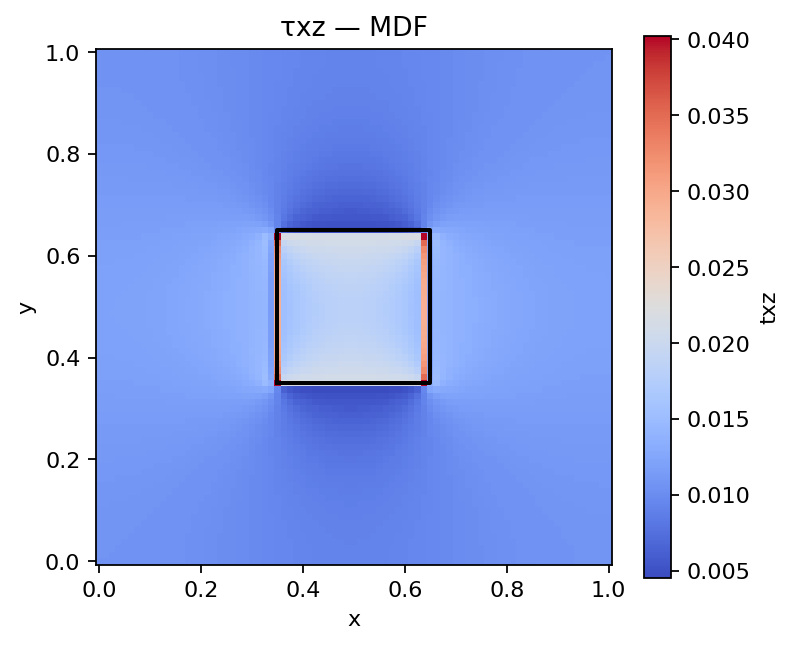
\includegraphics[width=\linewidth]{Template_with_Instructions_for_Preparing_Manuscripts_for_Trends_in_Computational_and_Applied_Mathematics/mdf.png}
        \caption*{(a)}
    \end{minipage}
    \hfill
    \begin{minipage}{0.47\textwidth}
        \centering
        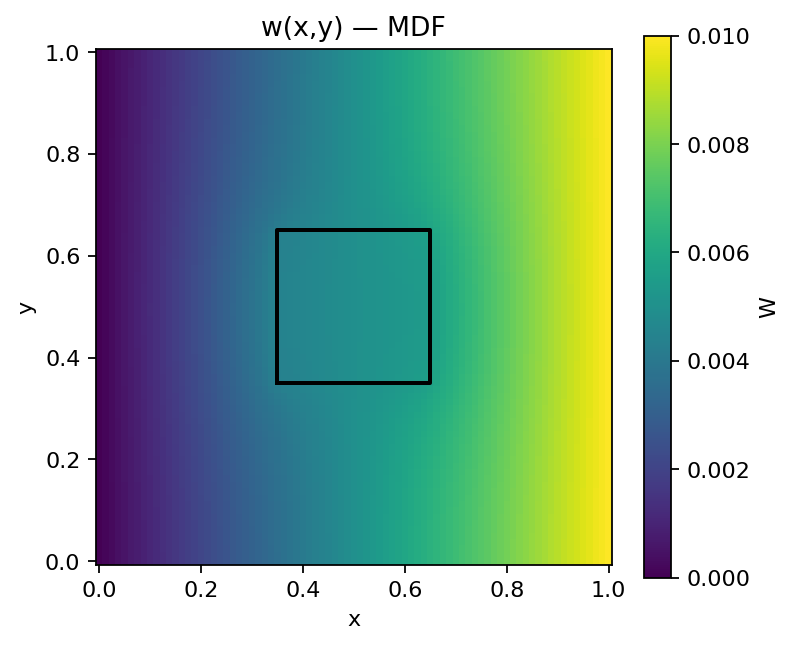
\includegraphics[width=\linewidth]{mdf2.png}
        \caption*{(b)}
    \end{minipage}
    \caption{Comparação dos resultados obtidos pelo método das diferenças finitas.}
    \label{fig:comparacao_mdf}
\end{figure}

Podemos observar como a tensão de cisalhamento é maior na inclusão, e o deslocamento aumenta conforme se afasta da origem.

Já para a simulação obtida através do Método de Elementos Finitos, os resultados foram bem próximos e podem ser observados na Figura \ref{fig:mef}.
\begin{figure}[h]
    \centering
    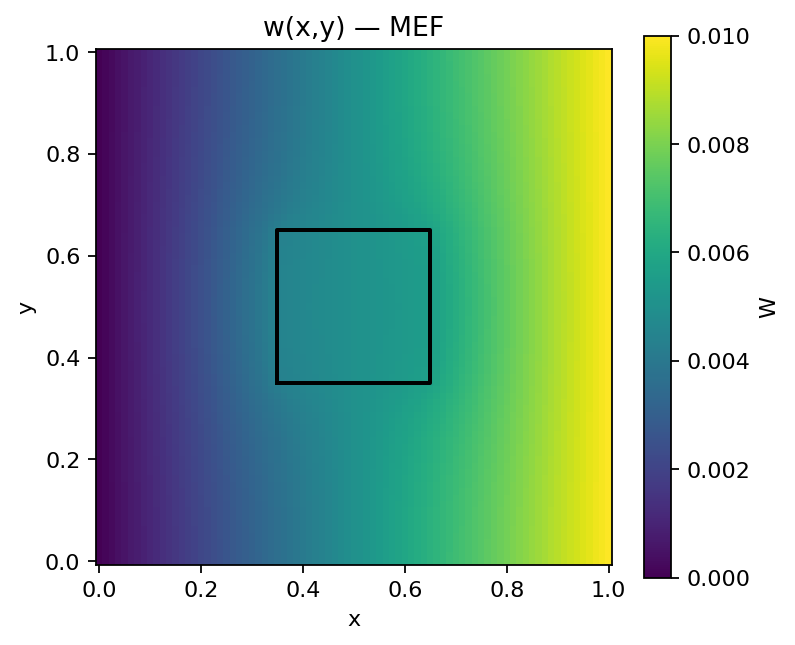
\includegraphics[width=0.5\linewidth]{mef.png}
    \caption{Resultado obtido através do método de elementos finitos}
    \label{fig:mef}
\end{figure}

\subsection{Erros relativos em norma $L^2$}

Tomando o MDF como referência, os erros relativos em norma $L^2$ para os campos
$w$, $\tau_{xz}$ e $\tau_{yz}$ foram avaliados na malha $81{\times}81$.
O MEF apresenta desvios da ordem de $10^{-3}$ ou menores em todos os campos.
A PINN apresenta desvios maiores nas tensões (ordem $10^{-2}$ a $10^{-1}$),
refletindo a dificuldade da rede em capturar descontinuidades de gradiente mesmo
com a decomposição de domínio. Esses resultados são ilustrados na
Figura~\ref{fig:erro}.

A Figura \ref{fig:erro} mostra o erro relativo entre o Método de Elementos finitos e o resultado obtido pela PINN.
\begin{figure}
    \centering
    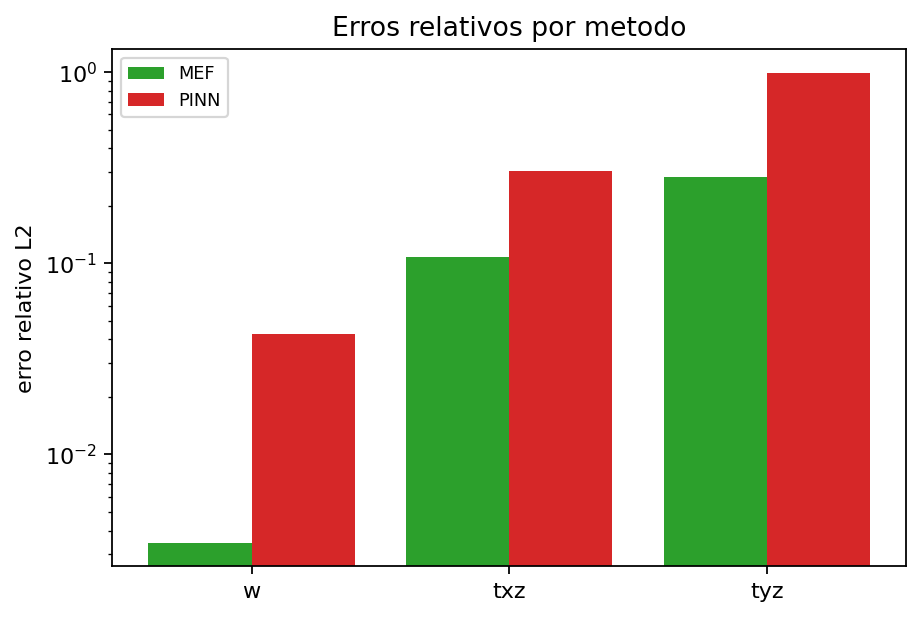
\includegraphics[width=0.5\linewidth]{erro.png}
    \caption{Erro relativo entre MEF e PINN.}
    \label{fig:erro}
\end{figure}

\subsection{Estudo paramétrico: razão de contraste $G_i/G_m$}

Com o solver MDF ($N=80$), variou-se a razão de contraste
$G_i/G_m \in \{1, 2, 5, 10, 50, 100\}$. O módulo efetivo $G_{ef}$ cresce
monotonicamente com o contraste e satura para razões elevadas, enquanto o pico de
tensão na interface $\max|\boldsymbol{\tau}|$ aumenta de forma expressiva ---
comportamento fisicamente esperado para inclusões progressivamente mais rígidas.

%*************************************************************
% DATA AVAILABILITY - This section is mandatory
% CHOOSE ONE OPTION AND REMOVE THE OTHERS
\newpage
\section*{Dados}

\noindent The data that support the findings of this study are available at \\
colab.research.google.com/drive/1Upls2ADBT56eJOo0saDpWYGbnElThzTp\#scrollTo=673f453

\section{Conclusão}

Neste trabalho, comparou-se o desempenho de três abordagens numéricas — o Método de Diferenças Finitas (MDF), o Método de Elementos Finitos (MEF) e as Redes Neurais Informadas pela Física (PINNs) — na solução do problema de cisalhamento antiplano em um compósito bifásico com inclusão quadrada.

Na estimativa do módulo de cisalhamento efetivo, os três métodos apresentaram resultados concordantes, com $G_{ef} \approx 1{,}14$ para a razão de contraste $G_i/G_m = 5$. Esse acordo indica que abordagens de naturezas tão distintas convergem para a mesma propriedade homogeneizada quando aplicadas a uma quantidade de interesse de caráter integral, como é o caso do módulo efetivo.

A concordância entre MDF e MEF mostrou-se praticamente exata, com erros relativos em norma $L^2$ da ordem de $10^{-3}$ ou inferiores em todos os campos avaliados. O MEF destacou-se, ainda, pela melhor representação das tensões de interface, beneficiando-se da atribuição das propriedades materiais por elemento e da integração por quadratura de Gauss. As PINNs, por sua vez, reproduziram de forma satisfatória o campo de deslocamento global, mas apresentaram desvios mais expressivos nas tensões (da ordem de $10^{-2}$ a $10^{-1}$), concentrados nas proximidades das quinas da inclusão, onde o gradiente do deslocamento é descontínuo. Vale ressaltar que esses desvios persistiram mesmo com a estratégia de decomposição de domínio e o acoplamento explícito do fluxo na interface \cite{jagtap2020conservative}, evidenciando a dificuldade intrínseca das redes em capturar singularidades de gradiente.

O estudo paramétrico, conduzido com o solver MDF, mostrou que o módulo efetivo cresce monotonicamente com a razão de contraste $G_i/G_m$ e satura para razões elevadas, enquanto o pico de tensão na interface aumenta de forma expressiva — comportamento fisicamente esperado para inclusões progressivamente mais rígidas.

Conclui-se, portanto, que os métodos clássicos de discretização permanecem mais precisos e robustos para problemas determinísticos de interface, sobretudo quando o objetivo é a captura acurada das tensões locais. As PINNs \cite{raissi2019pinn}, por outro lado, oferecem um paradigma flexível e livre de malha para a homogeneização computacional, particularmente atraente em cenários com geometrias complexas, problemas inversos ou estudos paramétricos, ainda que ao custo de menor acurácia nas regiões de gradiente acentuado.

Como perspectivas de trabalhos futuros, destacam-se o tratamento dedicado das singularidades nas quinas da inclusão — por meio de amostragem adaptativa, ponderação local da função de perda ou imposição forte das condições de interface —, a investigação de diferentes geometrias e frações volumétricas de inclusão, a extensão da análise ao caso tridimensional e a aplicação das PINNs a problemas inversos de identificação de propriedades materiais.

\bibliographystyle{ieeetr}
\bibliography{TCAM_bibliography}

\end{document}
